\documentclass[aps,prx,reprint,superscriptaddress,floatfix]{revtex4-2}

\usepackage[T1]{fontenc}
\usepackage{amsmath,amssymb,amsfonts,amsthm,bm}
\usepackage{booktabs,array,multirow}
\usepackage{graphicx}
\usepackage{microtype}
\usepackage[colorlinks=true,allcolors=blue]{hyperref}
\usepackage{url}
\usepackage{xspace}

\newtheorem{theorem}{Theorem}[section]
\newtheorem{proposition}[theorem]{Proposition}
\newtheorem{lemma}[theorem]{Lemma}
\newtheorem{corollary}[theorem]{Corollary}
\newtheorem{assumption}[theorem]{Assumption}
\newcommand{\E}{\mathbb{E}}
\newcommand{\Pp}{\mathbb{P}}
\newcommand{\R}{\mathbb{R}}
\newcommand{\J}{\mathbf{J}}
\newcommand{\M}{\mathbf{M}}
\newcommand{\W}{\mathbf{W}}
\newcommand{\Q}{\mathbf{Q}}
\newcommand{\I}{\mathbf{I}}
\newcommand{\trans}{\mathsf{T}}
\newcommand{\norm}[1]{\left\lVert #1\right\rVert}
\newcommand{\RSQ}{\textsc{RSQ}\xspace}

\hypersetup{
  pdftitle={Task-Weighted Observable Subspaces for Repeated Multi-Angle QAOA},
  pdfauthor={Molena Huynh},
  pdfsubject={A matrix-free construction and matched resource audit},
  pdfkeywords={QAOA, randomized numerical linear algebra, active subspaces, resource accounting}
}

\begin{document}

\title{Task-Weighted Observable Subspaces for Repeated Multi-Angle QAOA}
\author{Molena Huynh}
\email{molena.huynh@jmp.com}
\affiliation{North Carolina State University, Raleigh, North Carolina 27695, USA}
\date{July 2026}

\begin{abstract}
Repeated optimization on a graph changes task weights while preserving the
circuit and its observable geometry.  We formulate this setting as
task-weighted dimension reduction for multi-angle QAOA.  For observable
Jacobian $\J$ and task second moment
$\M=\E[ww^{\trans}]=LL^{\trans}$, the leading singular subspace of
$\J^{\trans}L$ minimizes expected discarded local gradient energy.  A
randomized algorithm constructs the subspace from Jacobian-vector and
vector-Jacobian actions; a residual diagnostic governs refreshes.  We audit
scalar objectives, vector observables, shots, checks, refreshes, and simulator
derivatives separately.  Across 16 graph-depth cells, residual-gated reuse
changes mean approximation ratio by $-1.57\pm1.04$ percentage points relative
to full-space SPSA while using $1.218$ times as many circuit evaluations, so
the criterion fails.  A 256-shot objective pilot favors per-task refresh by
$+0.61\pm1.57$ points but retains exact simulator-assisted construction.  The
evidence establishes the local representation and its reproducible cost
ledger, not query, hardware, scaling, or quantum advantage.
\end{abstract}
\keywords{quantum approximate optimization, multi-angle QAOA, randomized
linear algebra, active subspaces, resource accounting, reproducibility}
\maketitle

\section{Introduction}

The quantum approximate optimization algorithm (QAOA) alternates
problem-separating and mixing unitaries before optimizing their angles with a
classical routine \citep{farhi2014qaoa,hadfield2019alternating}.  It is a
canonical variational quantum algorithm because every outer-loop decision
changes the number of circuit preparations required to reach a useful
objective value \citep{peruzzo2014variational,mcclean2016theory}.  This
interaction is particularly important in the noisy intermediate-scale regime,
where circuit depth, sampling noise, and classical search all constrain
practical evidence \citep{preskill2018quantum,bharti2022noisy}.

Standard QAOA uses two angles per layer.  Multi-angle QAOA assigns separate
phase angles to cost terms and separate mixer angles to vertices, yielding
$d=p(|E|+|V|)$ coordinates at depth $p$ \citep{herrman2022multiangle}.  The larger parameterization can
increase expressivity, but a high-dimensional parameter vector need not imply
that every direction changes the observables relevant to a task
\citep{cerezo2021variational,zhou2020qaoa}.  Concentration and transfer
phenomena further suggest that useful structure can recur across related
instances or objectives \citep{brandao2018fixed,akshay2021concentration}.

We study a repeated-task regime on a fixed graph.  Let
$F(\bm\theta)\in\R^m$ collect the expected edge-cut observables and let a task
be $C_w(\bm\theta)=w^{\trans}F(\bm\theta)$.  Only $w$ changes between tasks.
Weighted-MaxCut transfer and warm-start studies motivate reuse, but do not
identify which local parameter directions preserve a distribution of weighted
objectives \citep{egger2021warm,shaydulin2023weighted}.  Graph-based
initialization methods similarly transfer angle information without solving
this observable-space problem \citep{jain2022gnn}.

The distinction matters because a scalar objective can hide the physical and
statistical cost of representation learning.  A single reverse-mode
vector-Jacobian product returns $\J^{\trans}w$ on a differentiable simulator,
whereas a device must estimate observables through measurements or
parameter-shift evaluations \citep{schuld2019evaluating,wierichs2022general}.
Simultaneous perturbation stochastic approximation (SPSA) uses two scalar
objective evaluations per update in either the full or reduced space
\citep{spall1992spsa}.  Consequently, a lower optimized dimension does not
automatically reduce the number of quantum queries.

Optimization can also become intrinsically difficult when gradients
concentrate near zero \citep{mcclean2018barren}.  Expressibility and control
structure affect this phenomenon \citep{holmes2022connecting,larocca2022diagnosing},
and gradient-free optimization does not remove it \citep{arrasmith2021effect}.
Any proposed reduction must therefore separate a mathematical statement about
retained local gradient energy from an empirical statement about end-to-end
optimization.

Our construction weights the observable Jacobian by the second moment of a
training task distribution.  It then applies fixed-precision randomized range
finding without forming the dense Jacobian \citep{halko2011finding,
martinsson2020randomized}.  The implementation follows blocked randomized QB
ideas \citep{yu2018randqb}, but its target matrix is the task-weighted
parameter sensitivity $A=\J^{\trans}L$ rather than a data matrix.

Figure~\ref{fig:protocol} summarizes the separation between basis-training
weights, evaluation tasks, local construction, and the matched audit.  The
central conclusion is negative but informative: the task-weighted subspace is
well defined and empirically better than a random basis, yet the tested
refresh policies do not establish an operational advantage.

\begin{figure*}[t]
\centering
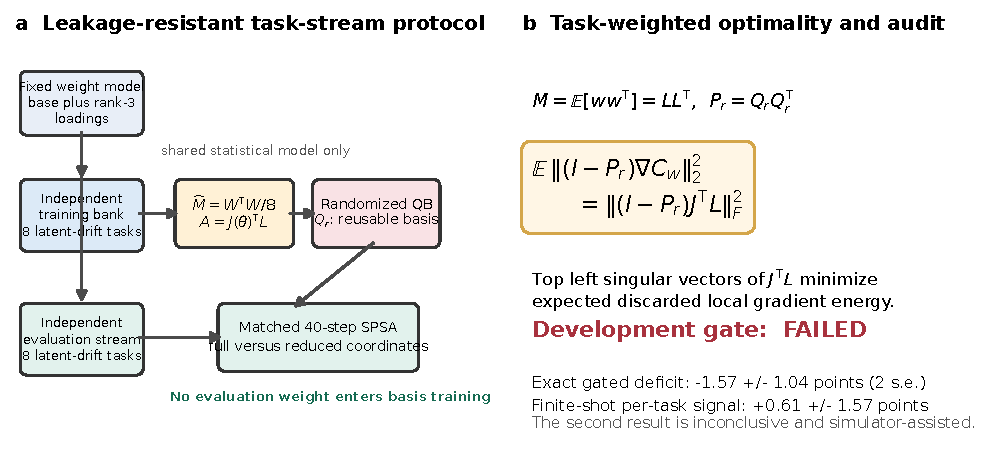
\includegraphics[width=0.98\textwidth]{figures/figure_amortized_protocol.pdf}
\caption{\textbf{Leakage-resistant repeated-task protocol.}  A training bank
defines the empirical task second moment; an independent evaluation stream
tests transfer.  Randomized QB constructs a local basis from
$\J^{\trans}L$, and full and reduced SPSA receive the same 40-step schedule.
The displayed development decision is generated from the committed evidence.}
\label{fig:protocol}
\end{figure*}

Our contributions are fourfold.  First, we prove the exact optimality criterion
for task-weighted local subspaces.  Second, we give a matrix-free construction
and a complete resource ledger.  Third, we distinguish reusable geometry from
objective-conditioned refresh and compare both against matched controls.
Fourth, we publish a deterministic reproduction chain: numerical displays are
regenerated from frozen CSV and JSON records, while protocol schematics are
rendered deterministically from committed configuration metadata.

\section{Background}

\subsection{Multi-Angle QAOA}

For an undirected graph $G=(V,E)$ with $n=|V|$ and $m=|E|$, define the edge
operator $C_e=(I-Z_iZ_j)/2$ for $e=(i,j)$.  A depth-$p$ multi-angle state is
\begin{equation}
 |\psi(\bm\theta)\rangle =
 \prod_{\ell=1}^{p}
 \left[
 \prod_{i\in V}e^{-i\beta_{\ell i}X_i}
 \prod_{e\in E}e^{-i\gamma_{\ell e}C_e}
 \right]|+\rangle^{\otimes n}.
 \label{eq:state}
\end{equation}
The parameter vector contains $p(m+n)$ angles.  The vector observable and its
Jacobian are
\begin{equation}
 F(\bm\theta)=
 \big(\langle\psi(\bm\theta)|C_e|\psi(\bm\theta)\rangle\big)_{e\in E},
 \qquad
 \J(\bm\theta)=\frac{\partial F}{\partial\bm\theta}\in\R^{m\times d}.
 \label{eq:jacobian}
\end{equation}
Analytic differentiation can evaluate individual parameter derivatives
\citep{mari2021estimating}; quantum-natural-gradient methods instead change the
metric in which an update is chosen \citep{stokes2020quantum}.  Our object is
different: it is a low-dimensional Euclidean subspace of parameters chosen to
retain a distribution of scalarized observable gradients.

All MaxCut edge terms commute in the computational basis.  One bitstring
therefore updates every component of $F$, and many task scalarizations may be
computed from the same measurement batch.  This form of observable reuse is
related in spirit to predicting many properties from shared measurements
\citep{huang2020shadows}, but it does not require general shadow tomography
\citep{aaronson2018shadow}.

\subsection{Repeated Weighted Objectives}

Let $w\in\R^m$ be a random task weight with finite second moment.  Choose an
integer $q\ge1$ and $L\in\R^{m\times q}$ such that
\begin{equation}
 \M=\E[ww^{\trans}]=LL^{\trans}.
 \label{eq:moment}
\end{equation}
The scalar objective $C_w(\bm\theta)=w^{\trans}F(\bm\theta)$ has local
gradient
\begin{equation}
 \nabla C_w(\bm\theta)=\J(\bm\theta)^{\trans}w.
 \label{eq:chain}
\end{equation}
If $Q\in\R^{d\times r}$ is orthonormal and $P=QQ^{\trans}$, the quantity
\begin{equation}
 \mathcal L(P)=
 \E_w\norm{(\I-P)\nabla C_w(\bm\theta)}_2^2
 \label{eq:loss}
\end{equation}
measures discarded local gradient energy.  It does not measure global
suboptimality, and it changes when the anchor $\bm\theta$ moves.

Active-subspace methods also average gradient outer products
\citep{constantine2015active}.  Sufficient-dimension-reduction methods,
including sliced inverse regression, solve related but statistically distinct
projection problems \citep{li1991sliced}.  Regression graphics provides a
broader account of response-preserving low-dimensional views
\citep{cook1998regression}.  Here, the vector-observable factorization exposes
the projection target exactly:
\begin{equation}
 \mathcal L(P)=\norm{(\I-P)\J^{\trans}L}_F^2.
 \label{eq:factorloss}
\end{equation}

\subsection{Randomized Range Approximation}

Set $A=\J^{\trans}L\in\R^{d\times q}$.  A randomized range finder probes
$A\Omega$ and orthogonalizes the result; a blocked fixed-precision algorithm
adds directions until a residual estimator falls below tolerance
\citep{woodruff2014sketching}.  Deterministic streaming sketches offer another
route when rows arrive sequentially \citep{liberty2013simple}.  Concentration
inequalities justify probabilistic residual controls under explicit random
matrix assumptions \citep{tropp2015matrix}, but the one-probe operational
refresh rule used here is not promoted to such a bound.

The matrix is accessed through
\begin{equation}
 Av=\J^{\trans}(Lv),\qquad
 A^{\trans}u=L^{\trans}(\J u).
 \label{eq:actions}
\end{equation}
The first action is a vector-Jacobian product and the second is a
Jacobian-vector product.  Our exact-statevector implementation uses reverse
automatic differentiation for the former and central differences for the
latter.

The resulting task-index trajectories and refresh events are displayed in
Fig.~\ref{fig:streams}.

\begin{figure*}[t]
\centering
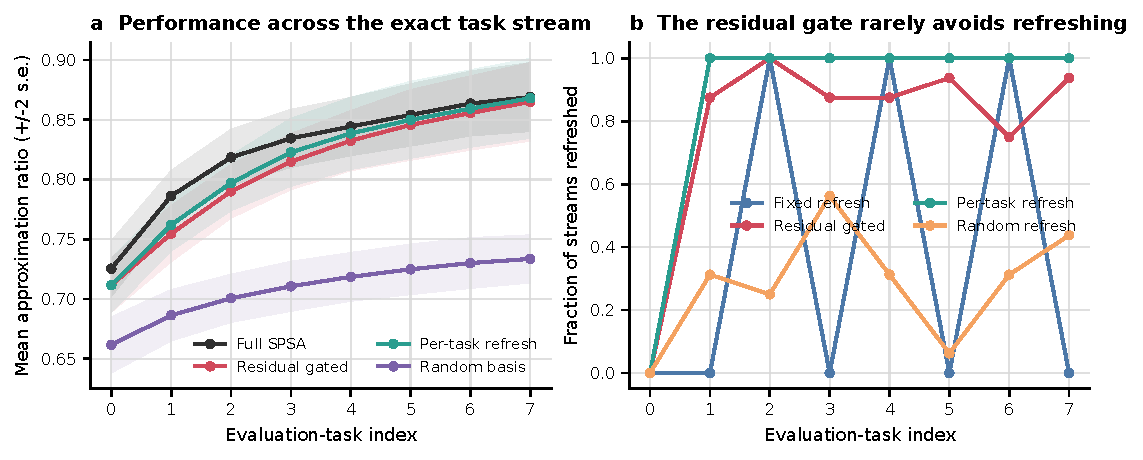
\includegraphics[width=0.98\textwidth]{figures/figure_amortized_stream.pdf}
\caption{\textbf{Evaluation-task trajectories.}  The left panel reports
task-index performance after nesting repeated measurements within a
graph-depth cell.  The right panel shows that residual gating refreshes on most
eligible transitions, limiting amortization in the tested regime.}
\label{fig:streams}
\end{figure*}

\section{Related Work}

Parameter concentration and interpolation can reduce the search needed by
QAOA without learning a new local basis \citep{zhou2020qaoa,
akshay2021concentration}.  Warm starts incorporate classical solutions
\citep{egger2021warm}, while learned optimizers predict search behavior from
training instances \citep{khairy2020learning}.  Broad optimizer studies show
that rankings depend on budget, noise, and objective geometry
\citep{bonet2023performance,montanez2025ramp}.

Graph representation learning provides invariant or equivariant features for
such transfer.  Graph convolutional networks aggregate normalized
neighborhoods \citep{kipf2017gcn}; graph attention assigns learned neighbor
weights \citep{velickovic2018gat}; and graph-isomorphism networks clarify the
discriminative power of message passing \citep{xu2019gin}.  Our basis is not a
graph embedding.  It is constructed within one graph from circuit
sensitivities and a task distribution.

The outer-loop optimization literature supplies several relevant controls.
Mesh-adaptive direct search is derivative free with a convergence framework
\citep{audet2006mesh}; BOBYQA builds a bounded quadratic interpolation model
\citep{powell2009bobyqa}; and covariance-matrix adaptation learns a search
distribution \citep{hansen2001cma}.  These methods alter the search strategy,
whereas \RSQ fixes the optimizer and changes only its coordinate subspace.

Bayesian optimization models an expensive response surface.  Efficient global
optimization introduced an improvement-based acquisition rule
\citep{jones1998efficient}; practical machine-learning variants made this
framework widely usable \citep{snoek2012practical}; and modern reviews organize
its modeling and acquisition choices \citep{shahriari2016taking}.  Batched
Monte Carlo acquisition functions can be implemented with differentiable
software \citep{balandat2020botorch}.  None of these eliminates the need to
count the quantum evaluations used to fit the surrogate.

Repeated tuning also resembles algorithm configuration.  Sequential
model-based configuration chooses settings from prior runs
\citep{hutter2011sequential}, while SMAC exposes a reproducible implementation
of this approach \citep{lindauer2022smac3}.  The classical algorithm-selection
problem is older and more general \citep{rice1976selection}.  It motivates our
use of disjoint training and evaluation streams, because reusing the same
tasks for basis choice and performance claims invites selection bias
\citep{cawley2010overfitting}.

Finally, the graph families in our experiments are controlled benchmarks:
Erd\H{o}s--R\'enyi random graphs \citep{erdos1959random}, preferential-attachment
graphs \citep{barabasi1999emergence}, and small-world constructions
\citep{watts1998collective}.  They are generated with NetworkX
\citep{hagberg2008networkx}.  Results on these small synthetic families do not
establish asymptotic or application-level generalization.

\section{Shortcomings of Static and Unweighted Subspaces}

\subsection{Inconsistency under Task Shift}

A static rank-$r$ subspace may preserve gradients for the training task
distribution and discard them under a shifted distribution.  The issue is
algebraic, not an artifact of randomized approximation.

\begin{theorem}[A shifted task can be completely discarded]
\label{thm:shift}
Fix an anchor with Jacobian $\J\in\R^{m\times d}$ and an orthogonal projector
$P$ of rank $r$.  If
$\operatorname{rank}(\J)>r$, then there exists a nonzero task weight
$w_\star\in\R^m$ such that
\[
 P\J^{\trans}w_\star=0
 \quad\text{and}\quad
 \J^{\trans}w_\star\ne0.
\]
Consequently, a distribution concentrated at $w_\star$ has unit relative
discarded gradient energy for $P$.
\end{theorem}

The full proof is in Appendix~\ref{app:proof-shift}.  The theorem does not say
that every shift is adversarial.  It says that no rank-deficient local
representation can be distribution free when the observable Jacobian has
larger rank.  Its construction permits signed scalarizations and therefore
does not, by itself, establish complete loss for task weights restricted to
the nonnegative orthant.  Monitoring principal-angle drift or retained energy
is necessary when the task law changes.

Classical statistical safeguards cannot repair an omitted physical direction
after the fact.  Bootstrap intervals describe sampling variation
\citep{efron1993bootstrap}; exact binomial limits quantify event rates
\citep{clopper1934fiducial}; and distribution-free inequalities can bound
bounded averages \citep{hoeffding1963probability}.  Each requires a sampling
model that is separate from the representation question.

\subsection{Refresh Bias and Hidden Physical Cost}

The residual diagnostic uses Gaussian directions $v_j$ and estimates
\begin{equation}
 \widehat\rho^2=
 \frac{\sum_{j=1}^{s}
 [D_{(\I-P)v_j}C_w(\bm\theta)]^2}
 {\sum_{j=1}^{s}[D_{v_j}C_w(\bm\theta)]^2}.
 \label{eq:gate}
\end{equation}
Its numerator and denominator estimate squared directional energies as the
finite-difference step vanishes, but their ratio is biased and the tested
$s=1$ rule is not a calibrated confidence statement.  Conformal prediction
offers distribution-free marginal coverage under exchangeability
\citep{vovk2005algorithmic,angelopoulos2021gentle}; conformalized quantile
regression adapts interval width to covariates \citep{romano2019cqr}; and
extensions handle some nonexchangeable settings \citep{barber2022exchangeability}.
Those results do not apply automatically to adaptively refreshed quantum
trajectories.

\begin{proposition}[Moments of exact residual probes]
\label{prop:probe-moments}
Let $C_w$ be differentiable at $\bm\theta$, write
$g=\nabla C_w(\bm\theta)$, let $P$ be an orthogonal projector, and let
$v_1,\ldots,v_s$ be independent $\mathcal N(0,\I)$ vectors.  For
\begin{align*}
 N_s&=\frac{1}{s}\sum_{j=1}^{s}
 [D_{(\I-P)v_j}C_w(\bm\theta)]^2,\\
 D_s&=\frac{1}{s}\sum_{j=1}^{s}
 [D_{v_j}C_w(\bm\theta)]^2,
\end{align*}
the exact directional derivatives satisfy
\begin{align}
 \E N_s&=\norm{(\I-P)g}_2^2,&
 \operatorname{Var}(N_s)&=\frac{2}{s}\norm{(\I-P)g}_2^4,\nonumber\\
 \E D_s&=\norm{g}_2^2,&
 \operatorname{Var}(D_s)&=\frac{2}{s}\norm{g}_2^4.
 \label{eq:probe-moments}
\end{align}
These moment identities do not imply that $N_s/D_s$ is unbiased; when
$g=0$, the target ratio is undefined.
\end{proposition}

Appendix~\ref{app:proof-probe-moments} proves the identities.  They isolate
Monte Carlo probe variability from finite-difference and finite-shot errors:
the implemented approximation inherits additional error terms not present in
Eq.~\eqref{eq:probe-moments}.

Cost accounting yields a second limitation.  Suppose a coordinate-gradient
method uses $2d$ circuit points per full update and $2r$ per reduced update,
there are $S$ updates per task and $K$ tasks, and basis construction plus
refreshes cost $C_{\rm basis}(K)$ circuit points across those tasks.

\begin{proposition}[Coordinate-gradient break-even condition]
\label{prop:breakeven}
Under the preceding ledger, let $S,K$ be positive integers, let
$0\le r<d$, and let $C_{\rm basis}(K)\ge0$.  The reduced method uses fewer
circuit points than the full method if and only if
\begin{equation}
 C_{\rm basis}(K)<2S(d-r)K.
 \label{eq:breakeven-implicit}
\end{equation}
If $C_{\rm basis}(K)=C_{\rm basis}$ is independent of $K$, this is equivalent
to
\begin{equation}
 K>\frac{C_{\rm basis}}{2S(d-r)}.
 \label{eq:breakeven}
\end{equation}
\end{proposition}

Appendix~\ref{app:proof-break} proves the equivalence.  It does not apply to
SPSA, because both coordinate systems use two perturbed objectives per update.
Nor may simulator VJPs be silently converted into hardware queries.

The matched exact-statevector audit is summarized graphically in
Fig.~\ref{fig:exactaudit}.

\begin{figure*}[t]
\centering
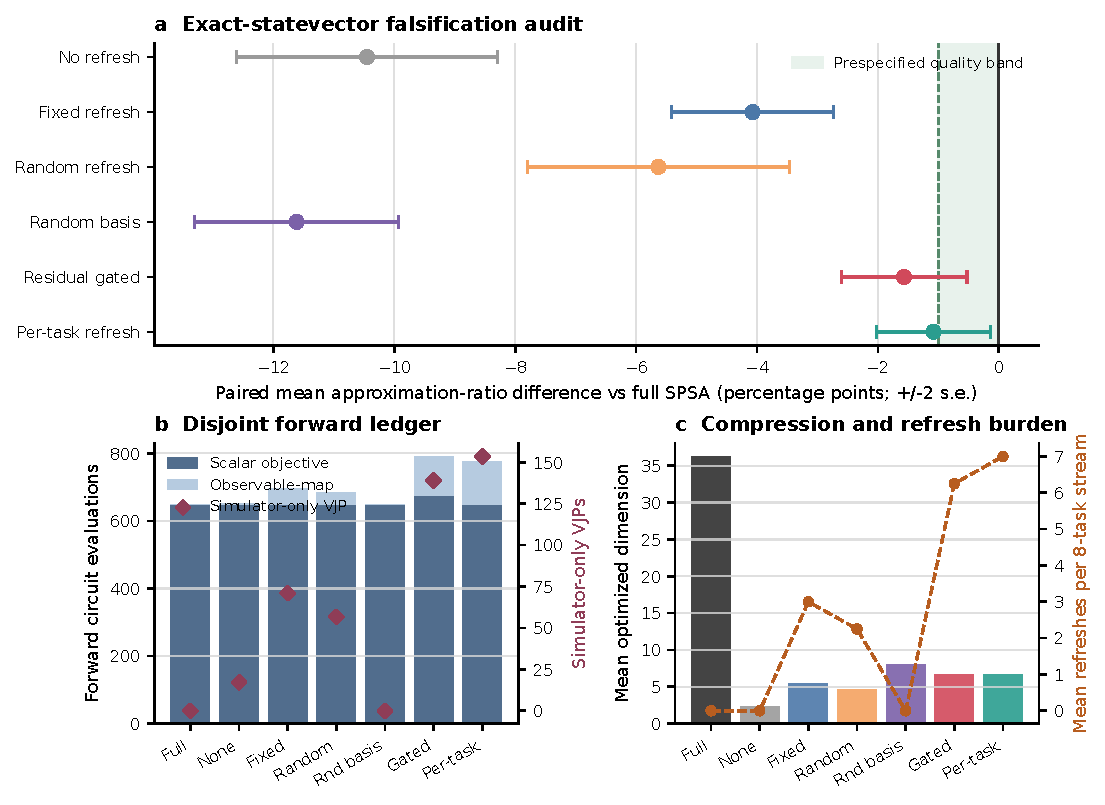
\includegraphics[width=0.98\textwidth]{figures/figure_amortized_exact_audit.pdf}
\caption{\textbf{Exact-statevector falsification audit.}  Residual-gated reuse
misses the declared one-percentage-point quality band and spends additional
observable evaluations and simulator VJPs.  Error bars are descriptive
$\pm2$ standard errors over configured graph-depth cells.}
\label{fig:exactaudit}
\end{figure*}

\subsection{No Scalar-Query Saving under Matched SPSA}

The preceding coordinate-gradient calculation does not transfer to an
optimizer whose query count is dimension independent.  For matched SPSA, a
subspace may change the search geometry, but it cannot reduce the two scalar
objectives used by each update.

\begin{proposition}[SPSA accounting obstruction]
\label{prop:spsa-accounting}
Suppose full-space and rank-$r$ SPSA each use $S$ updates and one final scalar
objective per task for $K$ tasks.  If the reduced method incurs nonnegative
basis, diagnostic, and refresh cost $C_{\rm basis}$ measured in additional
forward circuit points, then
\begin{equation}
 \begin{aligned}
 C_{\rm full}&=(2S+1)K,\\
 C_{\rm reduced}&=(2S+1)K+C_{\rm basis}\ge C_{\rm full}.
 \end{aligned}
 \label{eq:spsa-accounting}
\end{equation}
Equality holds if and only if $C_{\rm basis}=0$.
\end{proposition}

Appendix~\ref{app:proof-spsa-accounting} proves the statement from the SPSA
oracle ledger.  Thus any end-to-end saving in the present access model would
need fewer updates, cheaper per-objective measurement, or amortization over
some other resource; parameter compression alone is insufficient under the
matched stochastic-gradient and hardware-derivative access models considered
here \citep{spall1992spsa,schuld2019evaluating,wierichs2022general}.

\section{Task-Weighted Observable Subspaces}

\subsection{Optimal Task-Weighted Subspace}

\begin{theorem}[Optimal local parameter subspace]
\label{thm:optimal}
Let $w\in\R^m$ be square-integrable with
$\M=\E[ww^{\trans}]=LL^{\trans}$.  Fix a differentiable anchor with Jacobian
$\J\in\R^{m\times d}$, set $A=\J^{\trans}L$, and fix
$0\le r\le d$.  For every rank-$r$ orthogonal projector $P$,
\begin{equation}
 \E\norm{(\I-P)\J^{\trans}w}_2^2
 =\norm{(\I-P)A}_F^2.
 \label{eq:identity}
\end{equation}
If $A=U\Sigma V^{\trans}$ is a full singular-value decomposition with
$U\in\R^{d\times d}$, then
$P_r=U_rU_r^{\trans}$ minimizes this loss over all rank-$r$ orthogonal
projectors, and the minimum equals
$\sum_{j>r}\sigma_j(A)^2$.
\end{theorem}

Appendix~\ref{app:proof-optimal} gives a complete trace and variational proof.
The result is an exact population statement.  With training matrix
$\W\in\R^{K_{\rm tr}\times m}$, the implementation substitutes
\begin{equation}
 \widehat\M=K_{\rm tr}^{-1}\W^{\trans}\W,\qquad
 L=K_{\rm tr}^{-1/2}\W^{\trans},
 \label{eq:empiricalmoment}
\end{equation}
so the theorem holds exactly for the empirical task distribution.

The result is a local analogue of best low-rank approximation, but the
weighting is essential.  Unweighted observable sensitivity gives equal
importance to task directions that may never occur.  For $0<r<d$, the top
singular space is unique only when
$\sigma_r(A)>\sigma_{r+1}(A)$; otherwise every projector onto
an admissible leading invariant subspace attains the same loss.

\subsection{Matrix-Free Construction}

Blocked randomized QB starts from a Gaussian test block, applies the two
actions in Eq.~\eqref{eq:actions}, orthogonalizes against the accumulated
basis, and repeats until a relative residual condition or maximum rank is
reached.  Recycling initializes a new build from the previous basis but allows
rotation.  The method stores every stop reason, residual, rank, and operator
count.

The two-sided implementation uses simulator VJPs and finite-difference JVPs.
The forward-only control replaces VJPs by additional finite differences.  A
dense-SVD oracle materializes $\J$ and is reported separately rather than
treated as a deployable method.  This separation follows the broader principle
that randomized approximation quality and operator-access cost must be
reported together \citep{halko2011finding,woodruff2014sketching}.

\subsection{Residual-Gated Refresh}

The training task bank and evaluation stream share only a fixed latent weight
model.  Their random seeds and realized weights are disjoint.  At each
transition, one of six policies is applied: no refresh, fixed refresh,
residual-gated refresh, per-task refresh, random refresh, or a fixed isotropic
random basis.  The random-basis control isolates low dimension from learned
geometry; fixed and random refresh controls separate timing from content.

Multiple diagnostic comparisons are descriptive.  False-discovery-rate
procedures address families of statistical tests \citep{benjamini1995controlling},
and Neyman--Pearson testing formalizes simple-hypothesis power
\citep{neyman1933efficient}.  We do not retrofit either framework after
examining the development grid.  The only decision is the stated three-part
development gate.

\subsection{Matched Full and Reduced SPSA}

For native parameters or reduced coordinates $z$ with
$\bm\theta=\bm\theta_0+Qz$, SPSA draws a Rademacher perturbation $\delta_k$:
\begin{equation}
 \widehat g_k =
 \frac{C(x_k+c_k\delta_k)-C(x_k-c_k\delta_k)}
 {2c_k}\delta_k .
 \label{eq:spsa}
\end{equation}
Both matched SPSA update loops use 40 updates, identical gain schedules, one
perturbation pair per update, and one final objective, for 81
optimization-objective calls per task.  Residual diagnostics add separately
counted scalar calls to reduced methods.  The comparison therefore does not
claim that reduced SPSA saves objective queries.  Derivative-free methods can
respond differently to dimension and noise
\citep{audet2006mesh,hansen2001cma}; the matched design holds the optimizer
family fixed to isolate the representation.

\section{Experiments}

The benchmark asks whether task weighting retains more objective quality than
an isotropic rank-eight basis and whether residual-gated reuse stays within
one approximation-ratio point of matched full-space SPSA while using at most
$1.25$ times its forward circuit points.  The exact track crosses random
3-regular and Erd\H{o}s--R\'enyi graphs, $n\in\{8,10\}$, depths
$p\in\{1,2\}$, and graph seeds 41 and 42.  Each topology has eight basis
weights and an independent eight-task evaluation stream; graph-depth cells,
not optimizer iterates or measurement repeats, are the reported sampling
units.  The finite-shot pilot retains $p=2$, uses 256 shots per scalar
objective, and nests measurement seeds 0, 1, and 2 within each cell.  Neither
track contains gate noise, readout error, or hardware execution.

The controls are full SPSA, no refresh, fixed refresh, residual-gated refresh,
per-task refresh, random refresh, and a fixed isotropic random basis.  Matched
methods share initialization and optimizer seed schedules; every SPSA run uses
40 perturbation pairs and one terminal objective.  The primary endpoints are
the paired approximation-ratio difference from full SPSA and the disjoint
forward-cost ratio; residual energy, refresh counts, simulator JVPs/VJPs, and
shots are secondary diagnostics.  The displayed $\pm2$ standard errors are
descriptive over configured cells, and no confirmatory test is claimed.  The
conjunctive gate fails if any declared threshold fails.  Runs use Python
3.13.12, NumPy 2.4.3, PyTorch 2.11.0, NetworkX 3.6.1, and Matplotlib 3.10.8
on CPU.  From the repository root, \texttt{python run.py release} regenerates
summaries and displays, validates evidence and source synchronization, builds
the manuscript and source archive, and fails on drift.  The installed
\texttt{rsqaoa-reproduce-all} command provides immutable replay and seeded
reduced-cost execution.

\subsection{Exact-Statevector Repeated-Task Benchmark}

The exact grid contains random 3-regular and Erd\H{o}s--R\'enyi graphs with
$n\in\{8,10\}$, two graph seeds, and $p\in\{1,2\}$.  Eight topologies yield 16
configured topology-depth cells.  Each graph receives eight training weights
and an independent eight-task evaluation trajectory generated by a positive
rank-three latent model with autoregressive drift.  Weight vectors are
normalized to mean one.

The statevector backend uses complex-128 PyTorch tensors
\citep{paszke2019pytorch}.  Brute-force weighted MaxCut supplies the denominator
of each approximation ratio.  Results average tasks within a graph-depth cell;
paired differences subtract full SPSA in the same cell.  Since both depths
reuse each topology, the reported $\pm2$ standard errors are descriptive and
do not model cross-depth dependence.  Comparisons across multiple data sets
require care even under independent sampling \citep{demsar2006statistical}.

Table~\ref{tab:legacy} reports the legacy numerical summary, and
Fig.~\ref{fig:legacytradeoff} shows its compression--quality tradeoff.

\begin{table*}[t]
\centering
\caption{\textbf{Legacy single-objective benchmark.}  Values are regenerated
from \texttt{experiments/results/maxcut\_small.csv}.  This track tests local
compression on independent objectives and is not merged with the repeated-task
development decision.}
\label{tab:legacy}
\resizebox{\textwidth}{!}{\begin{tabular}{lrrrr}
\toprule
Method & Depth & Parameters & Approx. ratio & Paired change \\
\midrule
Full ma-QAOA & 1 & 23.7 & 0.862 $\pm$ 0.053 & -- \\
Symmetry-tied & 1 & 14.4 & 0.845 $\pm$ 0.065 & -1.67 $\pm$ 1.42 pp \\
Fixed-rank oracle & 1 & 8.0 & 0.764 $\pm$ 0.051 & -9.77 $\pm$ 2.09 pp \\
RSQ ($\varepsilon=0.01$) & 1 & 14.7 & 0.867 $\pm$ 0.051 & +0.48 $\pm$ 0.94 pp \\
RSQ ($\varepsilon=0.1$) & 1 & 14.7 & 0.862 $\pm$ 0.051 & -0.03 $\pm$ 0.79 pp \\
Forward-only RSQ & 1 & 8.0 & 0.798 $\pm$ 0.055 & -6.39 $\pm$ 1.98 pp \\
\addlinespace
Full ma-QAOA & 2 & 47.4 & 0.945 $\pm$ 0.044 & -- \\
Symmetry-tied & 2 & 28.7 & 0.940 $\pm$ 0.064 & -0.45 $\pm$ 2.64 pp \\
Fixed-rank oracle & 2 & 8.0 & 0.764 $\pm$ 0.048 & -18.07 $\pm$ 2.54 pp \\
RSQ ($\varepsilon=0.01$) & 2 & 14.7 & 0.897 $\pm$ 0.054 & -4.77 $\pm$ 2.47 pp \\
RSQ ($\varepsilon=0.1$) & 2 & 14.7 & 0.906 $\pm$ 0.058 & -3.88 $\pm$ 1.84 pp \\
Forward-only RSQ & 2 & 8.0 & 0.797 $\pm$ 0.053 & -14.73 $\pm$ 2.65 pp \\
\bottomrule
\end{tabular}
}
\end{table*}

\begin{figure*}[t]
\centering
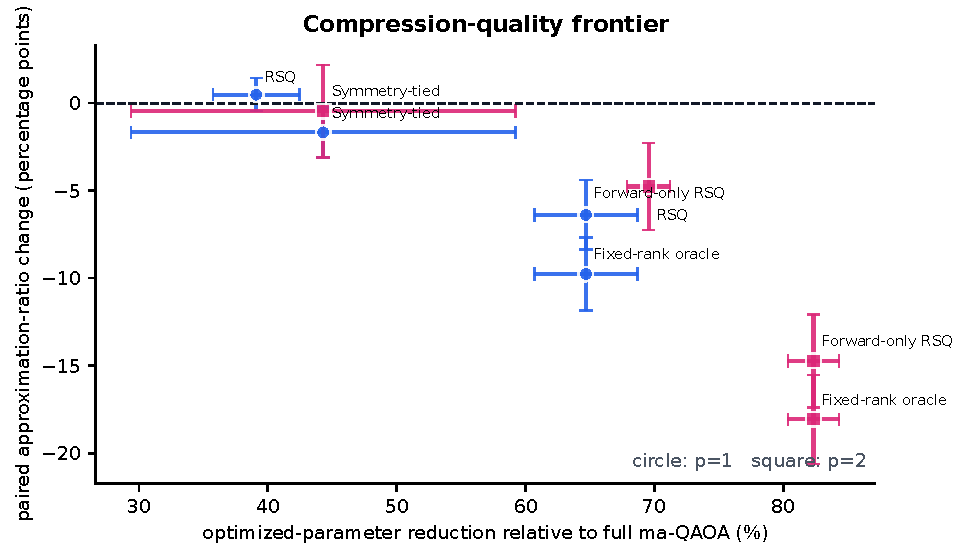
\includegraphics[width=0.98\textwidth]{figures/figure1_tradeoff.pdf}
\caption{\textbf{Legacy compression-quality tradeoff.}  The figure preserves
the original exact-statevector evidence track and exposes the stronger depth
dependence that motivated the repeated-task audit.}
\label{fig:legacytradeoff}
\end{figure*}

\subsection{Matched Development Audit}

The development gate requires the residual-gated method to be no more than one
approximation-ratio point below full SPSA, to exceed the random basis, and to
use at most $1.25$ times the forward circuit evaluations of full SPSA.  The
gated method achieves a paired difference of
$-1.57\pm1.04$ points and a cost ratio of $1.218$.  It beats the random basis
but fails the quality condition.  Per-task refresh gives
$-1.08\pm0.94$ points and uses still more construction.  The negative decision
is not changed by selecting the most favorable component.

Hyperparameter selection and final evaluation on the same grid can exaggerate
performance \citep{cawley2010overfitting}.  We therefore treat this experiment
as development only.  Standard bootstrap methodology could quantify
resampling uncertainty \citep{efron1993bootstrap}, but the small dependent
grid would still require an explicit topology-level sampling model.

The disjoint accounting categories used for the exact repeated-task audit are
reported in Table~\ref{tab:exact}.

\begin{table*}[t]
\centering
\caption{\textbf{Exact repeated-task audit.}  Objective and observable
evaluations are disjoint forward categories.  VJPs are simulator-only
operations and are not added to the forward total.}
\label{tab:exact}
\resizebox{\textwidth}{!}{\begin{tabular}{lrrrrrrr}
\toprule
Method & Ratio $\pm2\,$s.e. & $\Delta$ full (points) & Dim. & Obj. & Obs. & VJP & Refresh \\
\midrule
Full SPSA & 0.8244 $\pm$ 0.0230 & 0.00 (ref.) & 36.2 & 648 & 0.0 & 0.0 & 0.00 \\
No refresh & 0.7199 $\pm$ 0.0238 & -10.45 $\pm$ 2.16 & 2.4 & 648 & 4.8 & 17.1 & 0.00 \\
Fixed refresh & 0.7837 $\pm$ 0.0236 & -4.07 $\pm$ 1.34 & 5.5 & 648 & 46.8 & 71.0 & 3.00 \\
Residual gated & 0.8087 $\pm$ 0.0237 & -1.57 $\pm$ 1.04 & 6.6 & 676 & 113.2 & 138.9 & 6.25 \\
Per-task refresh & 0.8136 $\pm$ 0.0262 & -1.08 $\pm$ 0.94 & 6.7 & 648 & 128.0 & 153.5 & 7.00 \\
Random refresh & 0.7681 $\pm$ 0.0258 & -5.63 $\pm$ 2.17 & 4.7 & 648 & 34.8 & 56.6 & 2.25 \\
Random basis & 0.7083 $\pm$ 0.0202 & -11.62 $\pm$ 1.69 & 8.0 & 648 & 0.0 & 0.0 & 0.00 \\
\bottomrule
\end{tabular}
}
\end{table*}

\begin{figure*}[t]
\centering
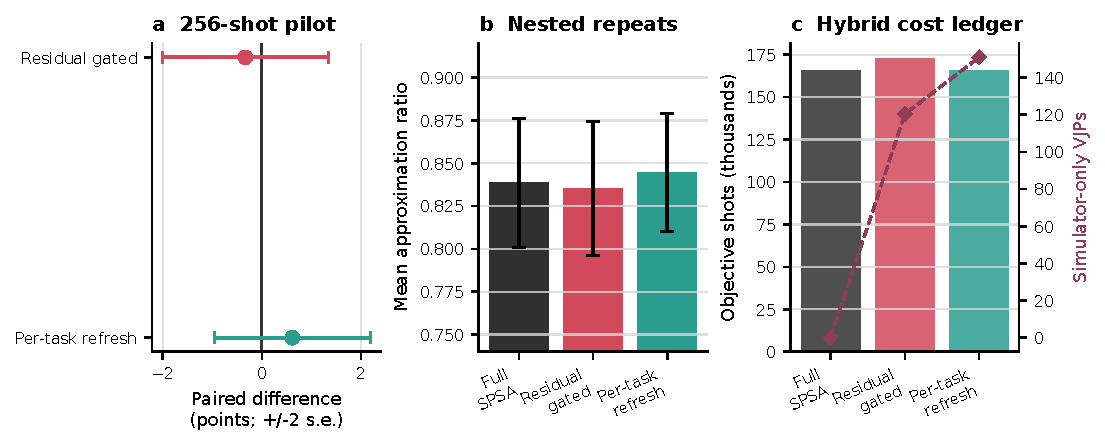
\includegraphics[width=0.98\textwidth]{figures/figure_amortized_shot_audit.pdf}
\caption{\textbf{Finite-shot objective pilot.}  Scalar objectives use 256
shots, while subspace construction remains exact and simulator-assisted.
Consequently, the figure is not an end-to-end hardware experiment.}
\label{fig:shotaudit}
\end{figure*}

\subsection{Finite-Shot Pilot}

Figure~\ref{fig:shotaudit} reports the finite-shot objective pilot under the
simulator-assisted subspace construction stated above.
The pilot retains $p=2$ and uses eight topology cells.  Each scalar objective
is estimated from 256 computational-basis shots, with three measurement
repeats nested inside each method-cell summary.  Candidate selection uses the
sampled objective, while the reported approximation ratio is the exact
expectation of the selected parameters.  This reduces reporting noise but
further separates the study from a hardware-only protocol.

Residual-gated reuse changes the mean by $-0.33\pm1.67$ points and per-task
refresh by $+0.61\pm1.57$ points relative to full SPSA.  Neither interval
resolves a stable advantage.  Exact binomial reasoning would be appropriate
for binary events under independent trials \citep{clopper1934fiducial}; it is
not a substitute for the continuous, paired, repeated-measurement analysis
used here.

The legacy family-stratified diagnostic is shown in
Fig.~\ref{fig:family}.

\begin{figure*}[t]
\centering
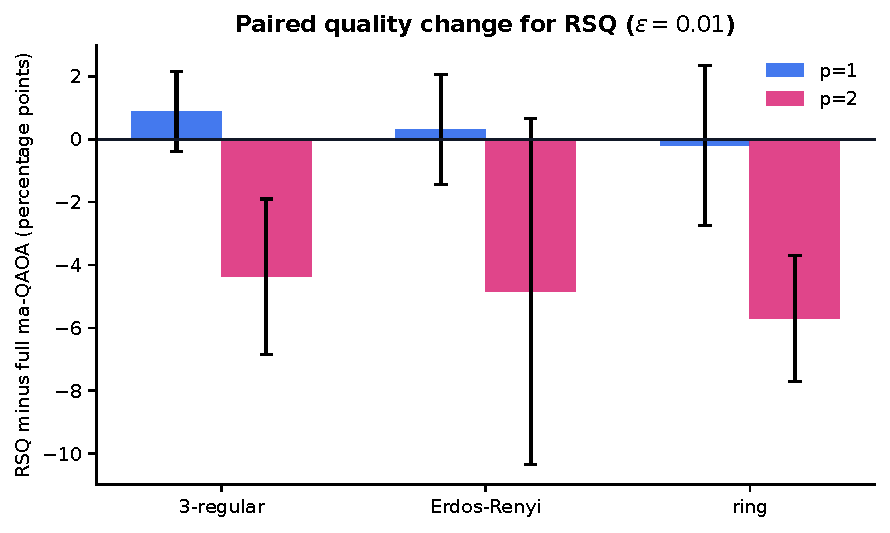
\includegraphics[width=0.98\textwidth]{figures/figure2_family.pdf}
\caption{\textbf{Legacy family-stratified behavior.}  Performance depends on
graph family and depth, so pooled averages are accompanied by stratified
diagnostics.}
\label{fig:family}
\end{figure*}

The experiment supports three conclusions.  First, task weighting identifies
a nonrandom local representation.  Second, refresh frequency is the dominant
obstacle to amortization on the tested short streams.  Third, the current
simulator-assisted construction cannot support a hardware-efficiency claim.
Longer task banks, larger graphs, calibrated refresh decisions, and
device-native sensitivity actions remain untested.

\section{Conclusion}

We derived a task-weighted observable tangent representation for repeated
multi-angle QAOA and proved its exact local optimality.  Matrix-free randomized
QB avoids dense Jacobian materialization and exposes every sensitivity action.
The representation is mathematically useful, but the matched evidence rejects
the tested operational claim: residual-gated reuse misses the development
quality threshold, refreshes frequently, and spends additional forward
evaluations.

\section*{Limitations}
The study has five principal limitations.  It uses at most ten qubits and
depth two; its graph families are synthetic; its task law is a controlled
rank-three drift model; its uncertainty summaries are descriptive; and its
subspace construction uses exact simulator derivatives.  These limitations
exclude claims of quantum advantage, hardware advantage, asymptotic scaling,
or distribution-free transfer.  General lessons about experiment design
remain valid: comparisons should use matched optimizers, preserve failed
gates, report strata, and keep simulator operations distinct from physical
measurements.

A confirmatory design is included but deliberately unexecuted.  It specifies
40 new topology units, longer task streams, changepoints, independent-weight
stress tests, shot and readout perturbations, device-native coordinate
gradients, and dense-oracle controls.  Its decision rule must be frozen before
the outcomes are generated.  Distribution-free calibration is attractive only
when its exchangeability conditions are defensible \citep{angelopoulos2021gentle,
barber2022exchangeability}; otherwise the resulting coverage statement must be
qualified.

The installable package exposes \texttt{rsqaoa-experiment} for a direct run and
\texttt{rsqaoa-reproduce} for full evidence regeneration or validation.
Source records, protocol hashes, implementation hashes, and generated-asset
hashes are committed with the manuscript.  This makes every numerical table
and figure traceable without implying that deterministic rerunning removes
modeling uncertainty.

\section*{Data Availability}
All numerical evidence used in the figures and tables is included in the
public repository at
\url{https://github.com/thmolena/Randomized-Subspace-QAOA} under
\texttt{experiments/results}.  The display manifest records
the SHA-256 digest of every consumed result file, while the deterministic
source archive contains the manuscript and all displayed assets.  No external
or restricted dataset is required, and no hardware data were collected.

\section*{Code Availability}
The complete implementation, frozen configurations, tests, evidence
validators, display generator, and archive builder are included in the
repository.  Installing the repository with \texttt{pip install .} exposes
\texttt{rsqaoa-experiment} for configured studies and
\texttt{rsqaoa-reproduce-all} for immutable replay or seeded regeneration.
The wheel contains its own evidence bundle and is independent of the original
checkout.

\clearpage
\bibliographystyle{apsrev4-2}
\bibliography{refs}

\clearpage
\appendix

\section{Proofs}

\subsection{Proof for Theorem~\ref{thm:shift}}
\label{app:proof-shift}

\begin{proof}
Let $\mathcal R=\operatorname{range}(\J^{\trans})\subseteq\R^d$.  By
assumption, $\dim\mathcal R=\operatorname{rank}(\J)>r$.  The range of $P$ has
dimension $r$, so
\[
 \dim(\mathcal R\cap\ker P)
 \ge \dim\mathcal R+\dim\ker P-d
 =\operatorname{rank}(\J)-r>0.
\]
Choose a nonzero $g\in\mathcal R\cap\ker P$.  Since
$g\in\operatorname{range}(\J^{\trans})$, there exists
$w_\star\in\R^m$ such that $\J^{\trans}w_\star=g$.  Because $g\ne0$, this
weight is not in $\ker(\J^{\trans})$.  Because $g\in\ker P$,
$P\J^{\trans}w_\star=Pg=0$, while
$\J^{\trans}w_\star=g\ne0$.

Let the shifted task distribution place probability one on $w_\star$.  Then
\[
 \frac{\E\norm{(\I-P)\J^{\trans}w}_2^2}
 {\E\norm{\J^{\trans}w}_2^2}
 =\frac{\norm{(\I-P)g}_2^2}{\norm g_2^2}
 =\frac{\norm g_2^2}{\norm g_2^2}=1,
\]
where $(\I-P)g=g$ because $Pg=0$.  This proves the claim.
\end{proof}

\subsection{Proof for Proposition~\ref{prop:probe-moments}}
\label{app:proof-probe-moments}

\begin{proof}
Differentiability gives
$D_uC_w(\bm\theta)=g^{\trans}u$ for every direction $u$.  Since $P$ is
orthogonal, $\I-P$ is symmetric, and therefore
\[
 D_{(\I-P)v_j}C_w(\bm\theta)
 =g^{\trans}(\I-P)v_j
 =((\I-P)g)^{\trans}v_j .
\]
Set $a=(\I-P)g$.  Rotational invariance of a standard Gaussian vector implies
$a^{\trans}v_j\sim\mathcal N(0,\norm a_2^2)$.  If
$Z\sim\mathcal N(0,\sigma^2)$, then
$\E Z^2=\sigma^2$ and $\E Z^4=3\sigma^4$, so
$\operatorname{Var}(Z^2)=\E Z^4-(\E Z^2)^2=2\sigma^4$.
Applying these identities with $\sigma^2=\norm a_2^2$ shows that each
summand of $N_s$ has mean $\norm a_2^2$ and variance
$2\norm a_2^4$.  Independence of the probes then gives
\[
 \E N_s=\norm a_2^2,\qquad
 \operatorname{Var}(N_s)
 =s^{-2}\sum_{j=1}^{s}2\norm a_2^4
 =\frac{2}{s}\norm a_2^4.
\]
Repeating the same calculation with $a=g$ proves the two identities for
$D_s$.  Finally, expectation does not commute with division, and $N_s$ and
$D_s$ are dependent because both use the same probes.  Thus the four moment
identities cannot establish $\E[N_s/D_s]=\E[N_s]/\E[D_s]$.  If $g=0$, both
population energies vanish and their relative ratio is not defined.
\end{proof}

\subsection{Proof for Proposition~\ref{prop:breakeven}}
\label{app:proof-break}

\begin{proof}
Under the stated ledger, $K$ tasks with $S$ full coordinate-gradient updates
use
\[
 C_{\rm full}=2dSK
\]
circuit points.  The reduced procedure uses $2r$ points per update plus the
complete basis and refresh cost:
\[
 C_{\rm reduced}=C_{\rm basis}(K)+2rSK.
\]
Thus $C_{\rm reduced}<C_{\rm full}$ is equivalent to
\[
 C_{\rm basis}(K)+2rSK<2dSK.
\]
Subtracting $2rSK$ from both sides gives
$C_{\rm basis}(K)<2S(d-r)K$, proving
Eq.~\eqref{eq:breakeven-implicit}.  When
$C_{\rm basis}(K)=C_{\rm basis}$ is independent of $K$, $S>0$ and $d-r>0$,
so division preserves the inequality and yields
\[
 K>\frac{C_{\rm basis}}{2S(d-r)}.
\]
Every algebraic step is reversible, proving both necessity and sufficiency.
\end{proof}

\subsection{Proof for Proposition~\ref{prop:spsa-accounting}}
\label{app:proof-spsa-accounting}

\begin{proof}
At each SPSA update, the algorithm evaluates the scalar objective at the two
parameter vectors
$x_k+c_k\delta_k$ and $x_k-c_k\delta_k$.  This count is two whether
$x_k\in\R^d$ represents full coordinates or
$x_k\in\R^r$ represents reduced coordinates.  After $S$ updates, either
method has therefore used $2S$ scalar objective evaluations.  Adding one
final evaluation of the selected iterate gives $2S+1$ evaluations per task
and $(2S+1)K$ evaluations across $K$ tasks.

By definition, $C_{\rm basis}$ contains every additional forward circuit point
used to construct a basis, evaluate a residual diagnostic, or refresh the
basis.  These points are not among the matched SPSA perturbation pairs or
final objectives.  Hence disjoint accounting gives
\[
 C_{\rm reduced}=(2S+1)K+C_{\rm basis},
 \qquad C_{\rm full}=(2S+1)K.
\]
The assumed nonnegativity $C_{\rm basis}\ge0$ yields
$C_{\rm reduced}\ge C_{\rm full}$.  Subtracting the two expressions gives
$C_{\rm reduced}-C_{\rm full}=C_{\rm basis}$, so equality holds exactly when
$C_{\rm basis}=0$.
\end{proof}

\subsection{Proof for Theorem~\ref{thm:optimal}}
\label{app:proof-optimal}

\begin{proof}
Let $P=P^{\trans}=P^2$ be any rank-$r$ orthogonal projector.  From
$\nabla C_w=\J^{\trans}w$,
\begin{align}
 \E\norm{(\I-P)\J^{\trans}w}_2^2
 &=\E\!\left[
 w^{\trans}\J(\I-P)^{\trans}(\I-P)\J^{\trans}w
 \right] \nonumber\\
 &=\operatorname{tr}\!\left(
 \J(\I-P)\J^{\trans}\E[ww^{\trans}]
 \right) \nonumber\\
 &=\operatorname{tr}\!\left(
 (\I-P)\J^{\trans}LL^{\trans}\J(\I-P)
 \right) \nonumber\\
 &=\operatorname{tr}\!\left(
 (\I-P)AA^{\trans}(\I-P)
 \right) \nonumber\\
 &=\norm{(\I-P)A}_F^2.
\end{align}
We used symmetry and idempotence in the second line and cyclic invariance of
trace in the third.

Let $A=U\Sigma V^{\trans}$ be a full singular-value decomposition with
$U\in\R^{d\times d}$, and write the eigenvalues of
$AA^{\trans}$ as $\lambda_j=\sigma_j(A)^2$ in nonincreasing order.  Since
\[
 \norm{(\I-P)A}_F^2
 =\operatorname{tr}(AA^{\trans})
  -\operatorname{tr}(PAA^{\trans}),
\]
minimizing the loss is equivalent to maximizing
$\operatorname{tr}(PAA^{\trans})$ over rank-$r$ projectors.  Write
$P=QQ^{\trans}$ with $Q^{\trans}Q=I_r$ and let
$B=U^{\trans}Q$.  Then $B^{\trans}B=I_r$ and
\[
 \operatorname{tr}(PAA^{\trans})
 =\operatorname{tr}\!\left(B^{\trans}
 \operatorname{diag}(\lambda_1,\ldots,\lambda_d)B\right)
 =\sum_{j=1}^{d}\lambda_j a_j,
\]
where $a_j=\sum_{k=1}^{r}B_{jk}^2$, $0\le a_j\le1$, and
$\sum_j a_j=r$.  Because the $\lambda_j$ are nonincreasing, a maximum of the
linear functional is attained at $a_j=1$ for $j\le r$ and $a_j=0$ for
$j>r$.  This value is attained by $Q=U_r$, hence by
$P_r=U_rU_r^{\trans}$.  The maximum retained energy is
$\sum_{j\le r}\sigma_j^2$, so the minimum discarded energy is
$\sum_{j>r}\sigma_j^2$.  This proves the theorem, including the
non-uniqueness when the boundary singular values are tied.
\end{proof}

\section{Algorithm}

\noindent\textbf{Matrix-free task-weighted QB procedure.}
Given an anchor $\bm\theta$, training weights $\W$, tolerance $\varepsilon$,
block size $b$, and maximum rank $r_{\max}$:
\begin{enumerate}
\item form the operator factor $L=K_{\rm tr}^{-1/2}\W^{\trans}$ without
forming $\widehat\M$;
\item expose $v\mapsto\J^{\trans}Lv$ and
$u\mapsto L^{\trans}\J u$;
\item draw a seeded Gaussian block $\Omega$ and compute
$Y=A\Omega$;
\item orthogonalize $Y$ twice against the recycled basis and the accumulated
new basis;
\item append nondegenerate orthonormal columns and estimate the relative
residual with independent probes;
\item stop at tolerance, rank exhaustion, or $r_{\max}$, recording the full
status; otherwise draw a new block and repeat.
\end{enumerate}
The two-pass orthogonalization controls numerical loss of orthogonality.  The
released status JSON records the rank and residual after every accepted block.

\section{Gradient-Free and Gradient-Based Methods}

The legacy benchmark compares full ma-QAOA, symmetry tying, a dense fixed-rank
oracle, two randomized tolerances, and an adjoint-free construction.
Figure~\ref{fig:operatorbudget} separates forward observable calls, JVPs,
VJPs, and dense Jacobian materializations.  These are overlapping operator
categories and must not be summed.

\begin{figure*}[t]
\centering
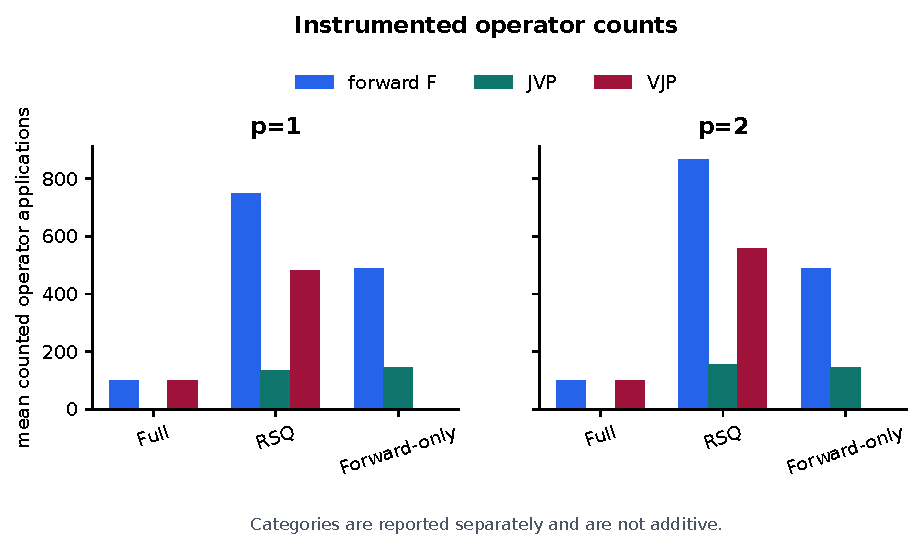
\includegraphics[width=0.98\textwidth]{figures/figure3_operator_budget.pdf}
\caption{\textbf{Operator-access ledger.}  Forward observable evaluations,
finite-difference JVPs, simulator VJPs, and dense-Jacobian events are reported
as distinct quantities.}
\label{fig:operatorbudget}
\end{figure*}

Gradient estimators on hardware can use parameter-shift identities
\citep{schuld2019evaluating,wierichs2022general}, while SPSA exchanges
coordinate resolution for two noisy function values per step
\citep{spall1992spsa}.  The released experiments do not equate these access
models.

\section{Bias and Variance of Refresh Decisions}

The diagnostic in Eq.~\eqref{eq:gate} is a ratio of random quadratic forms.
Even when its numerator and denominator are separately unbiased for scaled
gradient energies under exact directional derivatives, the ratio is not
unbiased.  Finite differences add truncation error, and finite-shot objectives
add measurement noise whose variance grows as the step shrinks.

The distribution of selected local ranks is shown in
Fig.~\ref{fig:rank}.

\begin{figure*}[t]
\centering
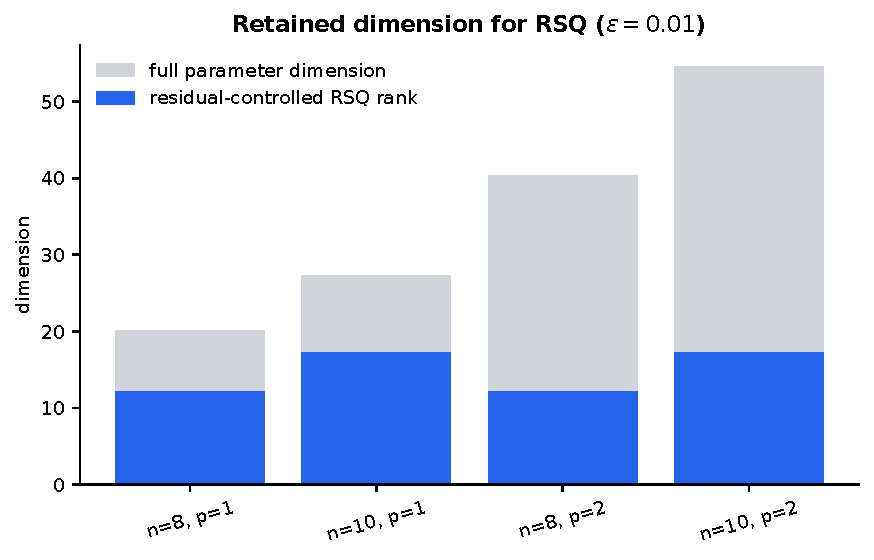
\includegraphics[width=0.98\textwidth]{figures/figure4_rank.pdf}
\caption{\textbf{Selected rank across the legacy grid.}  Rank adapts to the
local sensitivity spectrum but does not by itself predict end-to-end
efficiency.}
\label{fig:rank}
\end{figure*}

A calibrated next-task refresh rule would require a labeled quantity such as
the oracle benefit of rebuilding before that task.  Split calibration could
then be considered if calibration and future tasks were exchangeable
\citep{romano2019cqr}.  Online drift would require a different guarantee
\citep{barber2022exchangeability}.

\section{Repeated-Task Guidance Methods}

\subsection{No Refresh}
One basis is built at the initial anchor and reused for all eight tasks.  This
minimizes construction but is exposed to anchor and task drift.

\subsection{Fixed Refresh}
The basis is rebuilt after predetermined transitions.  Timing is independent
of observed residuals, which makes the policy a useful cost control.

\subsection{Residual-Gated Refresh}
Equation~\eqref{eq:gate} is evaluated on eligible transitions.  The tested
threshold frequently triggers, so its cost approaches per-task refresh.

\subsection{Per-Task Refresh}
Every transition rebuilds from the current anchor with recycled initialization.
This is the strongest local-adaptation control and the most construction-heavy.

\subsection{Random Refresh}
A seeded Bernoulli decision refreshes independently at each transition.  It
tests whether refresh count alone explains a gain.

\subsection{Random Basis}
A seeded isotropic rank-eight basis is fixed for the stream.  It tests whether
dimension reduction without learned sensitivity geometry is sufficient.

\section{Repeated-Task Benchmark Tasks}

\subsection{Regular Graphs}
Random 3-regular graphs provide degree-homogeneous topologies at $n=8$ and
$n=10$.

\subsection{Erd\H{o}s--R\'enyi Graphs}
Edges are sampled independently with probability $1/2$.  Fixed graph seeds
make the topology list reproducible.

\subsection{Low-Rank Weight Drift}
A positive base vector plus three orthonormal loadings defines the task family.
An AR(1) latent state with persistence $0.85$ and innovation scale $0.18$
produces training and evaluation streams with independent realizations.

\subsection{Independent Evaluation Stream}
No evaluation weight enters $\widehat\M$.  The shared base-and-loading law is
the stated transfer assumption; performance outside that law is unmeasured.

\subsection{Finite-Shot Objectives}
Computational-basis samples estimate all edge observables jointly.  The
subspace path remains exact, so this task is a hybrid diagnostic rather than a
device-native experiment.

\section{Experimental Details for the Exact Benchmark}

The declared development decision and the frozen repeated-task protocol appear
in Tables~\ref{tab:development-gate} and \ref{tab:protocol}, respectively.

\begin{table*}[t]
\centering
\caption{\textbf{Declared exact-development decision.}  The
residual-gated method passes the random-basis and forward-cost conditions but
fails the one-percentage-point quality condition, so the conjunction fails.}
\label{tab:development-gate}
\resizebox{\textwidth}{!}{\begin{tabular}{@{}lrrc@{}}
\toprule
Criterion & Required & Observed & Result \\
\midrule
Quality versus full SPSA & $\geq -0.010$ & -0.01567 & \textbf{fail} \\
Quality versus random basis & $>0$ & +0.10048 & pass \\
Forward-cost ratio versus full & $\leq 1.25$ & 1.21798 & pass \\
Conjunctive development gate & all pass & observed & \textbf{fail} \\
\bottomrule
\end{tabular}
}
\end{table*}

\begin{table*}[t]
\centering
\caption{\textbf{Frozen repeated-task protocol.}  Measurement repeats are
nested before graph-level aggregation.}
\label{tab:protocol}
\resizebox{\textwidth}{!}{\begin{tabular}{lrrrrl}
\toprule
Track & Topologies & Depths & Tasks & Repeats & Evaluator \\
\midrule
Exact development & 8 & 2 & 8 & 1 & exact statevector \\
Finite-shot pilot & 8 & 1 & 8 & 3 & 256 shots \\
\bottomrule
\end{tabular}
}
\end{table*}

Full and reduced SPSA use
$a_k=0.12/(k+6)^{0.602}$,
$c_k=0.10/(k+1)^{0.101}$, and a maximum update norm of $0.40$.
The basis builder uses maximum rank eight, block size two, relative tolerance
$0.10$, six norm probes, and four residual probes.  The refresh diagnostic uses
one probe, step $0.01$ in the exact track, step $0.10$ in the shot track, and
threshold $0.30$.

The corresponding finite-shot resource summary is given in
Table~\ref{tab:shot}.

\begin{table*}[t]
\centering
\caption{\textbf{Finite-shot repeated-task audit.}  ``Shots'' counts scalar
objective shots; the VJP column records simulator-only construction.}
\label{tab:shot}
\resizebox{\textwidth}{!}{\begin{tabular}{lrrrrrr}
\toprule
Method & Ratio $\pm2\,$s.e. & $\Delta$ full (points) & Forward & Shots & VJP & Refresh \\
\midrule
Full SPSA & 0.8387 $\pm$ 0.0376 & 0.00 (ref.) & 648.0 & 165888 & 0.0 & 0.00 \\
Residual gated & 0.8353 $\pm$ 0.0392 & -0.33 $\pm$ 1.67 & 771.7 & 173056 & 120.4 & 5.58 \\
Per-task refresh & 0.8448 $\pm$ 0.0345 & +0.61 $\pm$ 1.57 & 773.0 & 165888 & 150.9 & 7.00 \\
\bottomrule
\end{tabular}
}
\end{table*}

\section{Experimental Details for the Finite-Shot Pilot}

Each matched SPSA loop uses 81 optimization-objective points; residual-gated
checks add separately counted objective points.  Every such point uses 256
shots.  The three measurement repeats share the graph, task, and optimization
method but use independent measurement seeds.  Exact post-evaluation of the
selected candidate is used only for analysis.

Figure~\ref{fig:refreshfrequency} makes the refresh burden explicit across the
tested transitions.

\begin{figure*}[t]
\centering
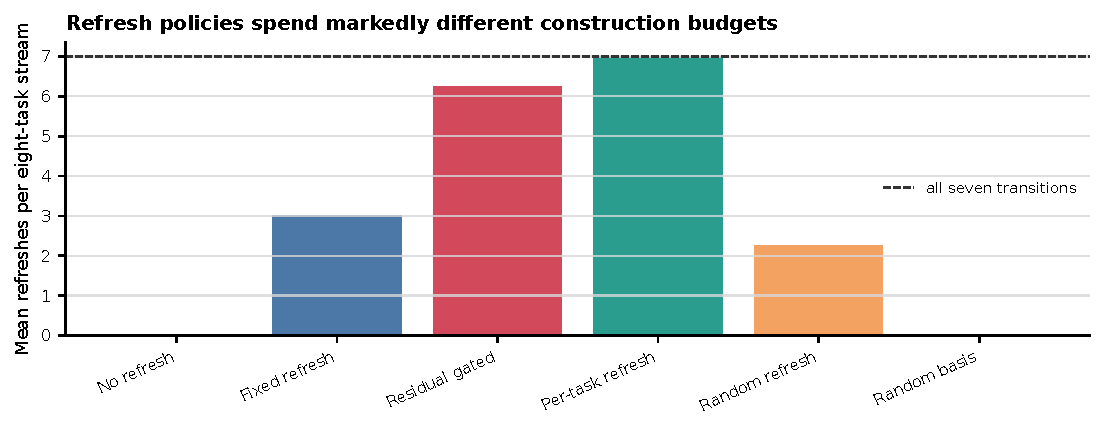
\includegraphics[width=0.98\textwidth]{figures/figure9_refresh_frequency.pdf}
\caption{\textbf{Refresh burden.}  The residual gate rebuilds on most of the
seven transitions, whereas fixed and random controls spend smaller
construction budgets.}
\label{fig:refreshfrequency}
\end{figure*}

\section{Physical Resource Accounting}

Every row records task-local and cumulative counts for scalar objective
points, vector-observable points, shots, JVPs, VJPs, builds, checks, refreshes,
and their disjoint forward total.  The ledger identities are validated before
display generation.

The display manifest records and validates SHA-256 values for the legacy CSV,
the exact and finite-shot task streams, and their three JSON summaries before
any figure is regenerated.  The audited paths are
\path{experiments/results/maxcut_small.csv},
\path{experiments/results/amortized_development.csv}, and
\path{experiments/results/amortized_shot_development.csv}, together with
their corresponding JSON summaries.

The released provenance record identifies every numerical source by a
repository-relative path and binds it to the full SHA-256 digest checked by
the display validator and packaged replay command.  Hash agreement establishes
source identity, not statistical validity.

The retained dimension by QAOA depth is reported in
Fig.~\ref{fig:dimensiondepth}.

\begin{figure*}[t]
\centering
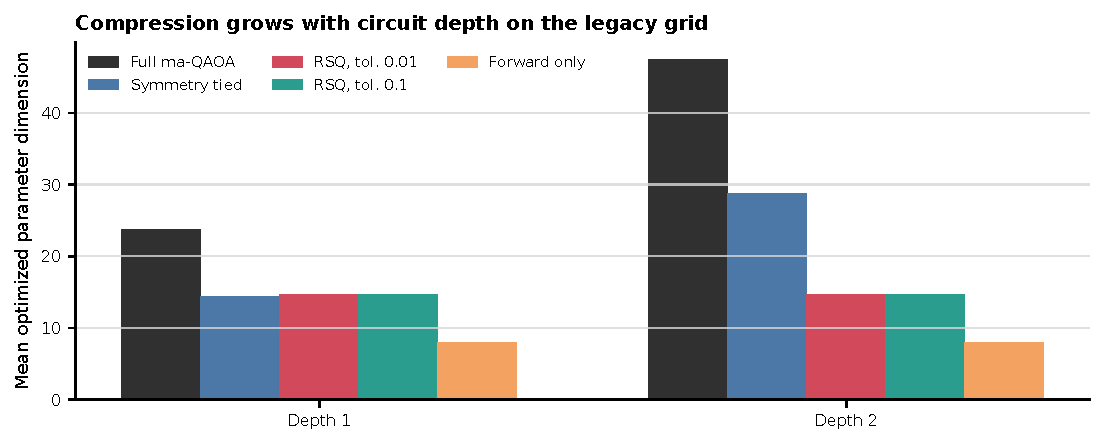
\includegraphics[width=0.98\textwidth]{figures/figure10_dimension_by_depth.pdf}
\caption{\textbf{Depth-dependent compression.}  The number of retained
directions grows more slowly than the ambient multi-angle dimension on this
small legacy grid.}
\label{fig:dimensiondepth}
\end{figure*}

\section{Additional Analysis}

The quality--cost frontier and family-conditional differences are displayed in
Figs.~\ref{fig:frontier} and \ref{fig:familyeffects}.

\begin{figure*}[t]
\centering
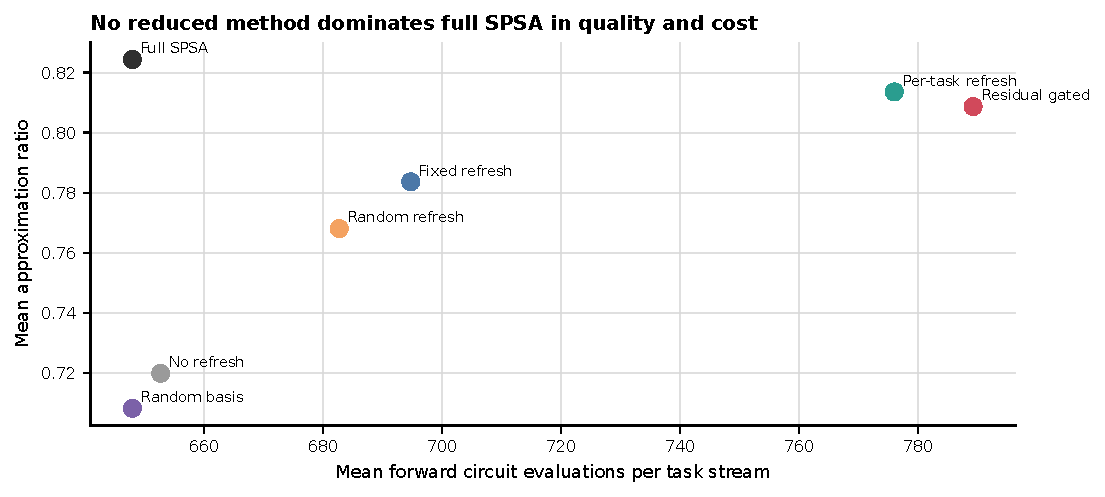
\includegraphics[width=0.98\textwidth]{figures/figure11_quality_cost_frontier.pdf}
\caption{\textbf{Quality-cost frontier.}  Mean forward cost includes scalar
and vector-observable points.  No reduced method simultaneously dominates full
SPSA in the development audit.}
\label{fig:frontier}
\end{figure*}

\begin{figure*}[t]
\centering
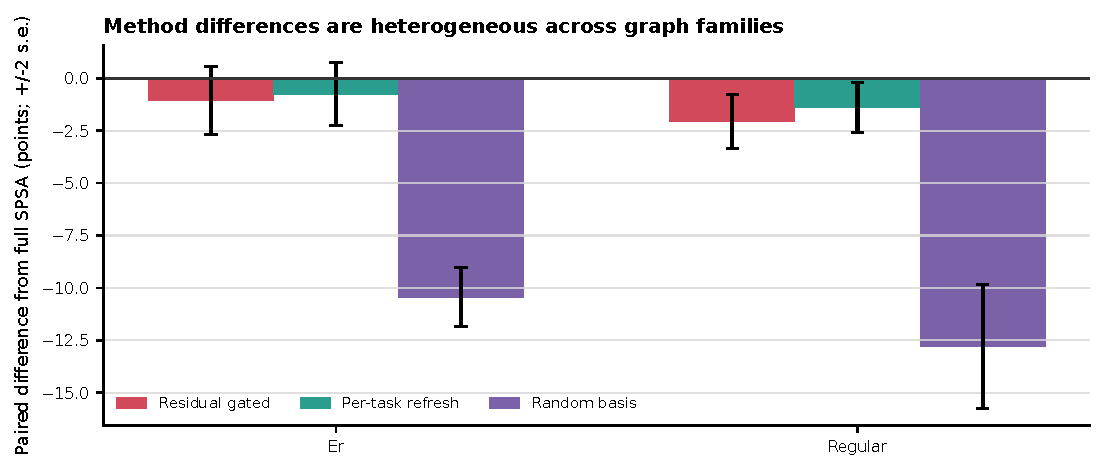
\includegraphics[width=0.98\textwidth]{figures/figure12_family_effects.pdf}
\caption{\textbf{Family heterogeneity.}  Paired method differences vary across
the configured graph generators; bars show descriptive $\pm2$ standard
errors.}
\label{fig:familyeffects}
\end{figure*}

The complete frozen-evidence reproduction chain is recorded in
Fig.~\ref{fig:reproductionmap}.

\begin{figure*}[t]
\centering
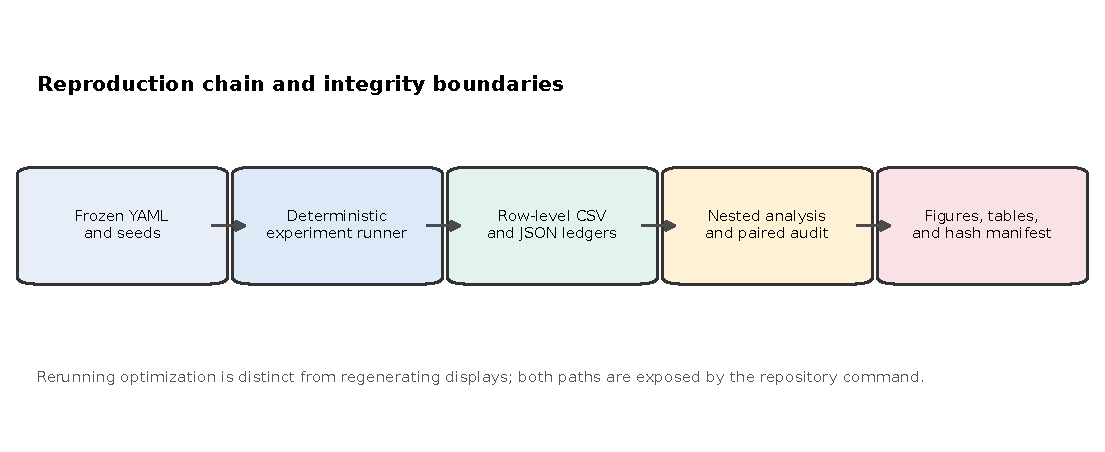
\includegraphics[width=0.98\textwidth]{figures/figure13_reproducibility_map.pdf}
\caption{\textbf{Reproduction chain.}  Frozen configurations and seeds produce
row-level evidence; analysis creates displays and a hash manifest.  Rerunning
optimization and regenerating displays remain distinct operations.}
\label{fig:reproductionmap}
\end{figure*}

The confirmatory design adds changepoints, independent task distributions,
longer streams, larger graphs, readout perturbations, and device-native
coordinate gradients.  Classical-shadow ideas may reduce the cost of broad
observable estimation in other operator families \citep{huang2020shadows};
they are unnecessary for the commuting MaxCut measurements used here.

\end{document}
